Shortly before she disappeared, Dr. Jonas was obsessed with studying the designs
found on the dice used by the ancient Heyting people. It seems that between
one and seven pips would be handcarved into the sides of a cube. While the position 
of the pips wouldn't affect the value of the roll (two pips always has a value of \(2\), 
no matter how they are arranged), some pip designs were considered
sacred, while the rest were known as profane.

I don't know the rules for what makes a pip design sacred or not, but I've attached
some examples from Dr. Jonas's notes. Maybe they'll be of some use in understanding
one of her journal entires. -BF

\begin{center}
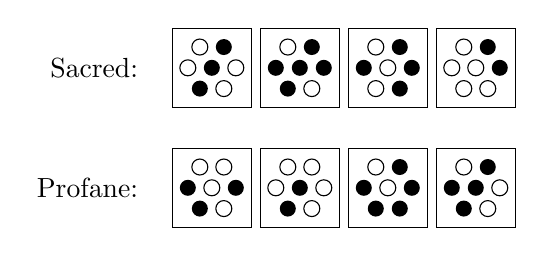
\begin{tikzpicture}[x=0.04in,y=0.04in]
\begin{scope}[shift={(0,0)}]
\node[anchor=east] at (-180:8) {Sacred:};
\draw (-45:7) rectangle (135:7);
\fill (0:0) circle (1);
\draw (0:3) circle (1);
\fill (60:3) circle (1);
\draw (120:3) circle (1);
\draw (180:3) circle (1);
\fill (-120:3) circle (1);
\draw (-60:3) circle (1);
\end{scope}
\begin{scope}[shift={(11,0)}]
\draw (-45:7) rectangle (135:7);
\fill (0:0) circle (1);
\fill (0:3) circle (1);
\fill (60:3) circle (1);
\draw (120:3) circle (1);
\fill (180:3) circle (1);
\fill (-120:3) circle (1);
\draw (-60:3) circle (1);
\end{scope}
\begin{scope}[shift={(22,0)}]
\draw (-45:7) rectangle (135:7);
\draw (0:0) circle (1);
\fill (0:3) circle (1);
\fill (60:3) circle (1);
\draw (120:3) circle (1);
\fill (180:3) circle (1);
\draw (-120:3) circle (1);
\fill (-60:3) circle (1);
\end{scope}
\begin{scope}[shift={(33,0)}]
\draw (-45:7) rectangle (135:7);
\draw (0:0) circle (1);
\fill (0:3) circle (1);
\fill (60:3) circle (1);
\draw (120:3) circle (1);
\draw (180:3) circle (1);
\draw (-120:3) circle (1);
\draw (-60:3) circle (1);
\end{scope}
\begin{scope}[shift={(0,-15)}]
\node[anchor=east] at (-180:8) {Profane:};
\draw (-45:7) rectangle (135:7);
\draw (0:0) circle (1);
\fill (0:3) circle (1);
\draw (60:3) circle (1);
\draw (120:3) circle (1);
\fill (180:3) circle (1);
\fill (-120:3) circle (1);
\draw (-60:3) circle (1);
\end{scope}
\begin{scope}[shift={(11,-15)}]
\draw (-45:7) rectangle (135:7);
\fill (0:0) circle (1);
\draw (0:3) circle (1);
\draw (60:3) circle (1);
\draw (120:3) circle (1);
\draw (180:3) circle (1);
\fill (-120:3) circle (1);
\draw (-60:3) circle (1);
\end{scope}
\begin{scope}[shift={(22,-15)}]
\draw (-45:7) rectangle (135:7);
\draw (0:0) circle (1);
\fill (0:3) circle (1);
\fill (60:3) circle (1);
\draw (120:3) circle (1);
\fill (180:3) circle (1);
\fill (-120:3) circle (1);
\fill (-60:3) circle (1);
\end{scope}
\begin{scope}[shift={(33,-15)}]
\draw (-45:7) rectangle (135:7);
\fill (0:0) circle (1);
\draw (0:3) circle (1);
\fill (60:3) circle (1);
\draw (120:3) circle (1);
\fill (180:3) circle (1);
\fill (-120:3) circle (1);
\draw (-60:3) circle (1);
\end{scope}
\end{tikzpicture}
\end{center}



%This mostly ordinary journal has strange doodles at the start of each line.
%In fact these are pictures of early dice from the Heyting people, or at least some of them are.
%Dr. Jonas was a Heyting expert, so there is no way she drew incorrect dice on accident.
%Both of the dates at the beginning look wrong as well.
%Dr. Jonas must have put them there for some other purpose.
